%!TEX root = ../template.tex
%Developed using Sublime Text 3 with LaTexTools plugin
%SUPER+b for compiling latex to pdf
%Don't forget to use SUPER+R to jump between top level commands!
%%%%%%%%%%%%%%%%%%%%%%%%%%%%%%%%%%%%%%%%%%%%%%%%%%%%%%%%%%%%%%%%%%%%
%% chapter2.tex
%% UNL thesis document file
%%
%% Chapter with the template manual
%%%%%%%%%%%%%%%%%%%%%%%%%%%%%%%%%%%%%%%%%%%%%%%%%%%%%%%%%%%%%%%%%%%%
\chapter{State of the Art}
\label{cha:state_of_the_art}
% ================
% = Introduction =
% ================

The most common methods used in the detection of turn insulation faults in \acrshort{ims} are those based on models and intelligent systems. As for model-based, the most conventionally used set of techniques are the \acrfull{esa}, while intelligent systems are presented in various 
procedures.

\acrshort{esa} is the general term for a set of electrical machine condition monitoring techniques through the analysis of electrical signals such as current and voltage. Several works report the use of those techniques applied to turn insulation fault detection, presented in section \ref{sec:conventional_techniques}. However, one issue that is rarely discussed is the need for rapid response to prevent catastrophic damage when an interturn short-circuit fault arises. This topic is addressed in section \ref{subsec:resolution_fast_response}.

The use of intelligent systems have gain a lot of momentum and are target of recent works, where the most related to this work are presented in section \ref{sec:machine_learning_approaches}.



\section{Conventional Techniques for fault detection} % (fold)
\label{sec:conventional_techniques}

\subsection{Machine Current Signature Analysis} % (fold)
\label{subsec:mcsa}
\acrfull{mcsa} is a technique used to analyze and monitor the trend of dynamic energized systems. This technique uses the induction motor as a transducer by monitoring the stator currents, allowing the user to analyze the produced power spectrum, referred as motor signature. This allows to get insights on the motors, by identifying the magnitude and frequency of each individual component that integrates the motor current signal, without the need to stop the motor.


\subsection{Park's Vector and Extended Park's Vector Approach} % (fold)
\label{subsec:epva}

Stator Winding Fault Diagnosis in Three-Phase Synchronous and Asynchronous Motors, by the Extended Park’s Vector Approach


\subsection{Park-Hilbert Method} % (fold)
\label{subsec:park_hilbert_method}

\subsection{Symmetrical Components under Stator Faults} % (fold)
\label{subsec:symmetrical_components}

\subsection{Negative Sequence Current Compensation} % (fold)
\label{subsec:negative_sequence_current_compensation}

\subsection{Zero Sequence Components} % (fold)
\label{subsec:zero_sequence_components}

\subsection{Resolution and Fast Response} % (fold)
\label{subsec:resolution_fast_response}

One issue that is rarely discussed is the need for a rapid response to prevent a catastrophic damage when an interturn short-circuit fault happens. For example, if the conventional fast Fourier transform (FFT) is used to detect faulty components in an early stage, an high-frequency resolution is required. This leads to long sampling periods, which could be longer than the time needed to prevent a catastrophic failure when the fault arises. 

As stated in ~\cite{Cheng2011}, an analysis on the trade off between resolution and fast response is needed. The authors of ~\cite{Cheng2011} use a sampling time of 0.25 seconds, which leads to a frequency resolution of 4Hz, for calculating the spectrum of the complex current vector to detect positive and negative sequence currents.

In this context, effective approaches need to use signal-processing techniques for achieving appropriate frequency resolution with short sampling periods. They should as well not have heavy computational complexities, so that processing almost in real time may be accomplishable ~\cite{Riera-Guasp2015}. 

\section{Intelligent Systems for fault detection} % (fold)
\label{sec:machine_learning_approaches}

\subsection{Artificial Neural Networks} % (fold)
\label{sec:ann}

\Acrfullpl{ann} are classifiers inspired by Biology. As all kind of classifiers, an \Acrshort{ann} goal is to maximize the likelihood for the predicted result of a given input to be as close as possible of the real result. This goal is accomplished by training the \Acrshort{ann} , which will adapt the consideration of the input against the expected result of that input. This classifier provides a general method for learning functions from examples, being the examples real-valued, discrete-valued, or vector-valued.

\Acrshort{ann} are composed by perceptrons, which are units that take a vector of real-valued inputs, calculates a linear combination of these inputs, and then computes a function which will give the result, as seen in figure \ref{fig:sigmoid_unit}.

\begin{figure}[htpb]
\centering
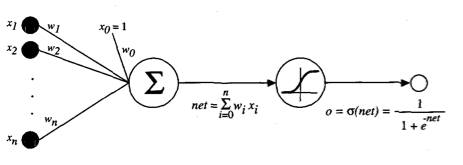
\includegraphics[width=0.5\textwidth]{sigmoidunit.png}
\caption{A perception unit with sigmoid activation function}
\label{fig:sigmoid_unit}
\end{figure}

Each perceptron have a linear combination so that a value may be produced from the input vector. from figure \ref{fig:sigmoid_unit}, it can be seen that each input has its own height. So, for example, a simple linear combination could be such as the equation \ref{eq:linear_combination}.

\begin{equation} 
\label{eq:linear_combination}
\sum_{i=1}^{n} w_{i}*x_{i}
\end{equation}

After the perceptron computes the linear combination, this value is applied to a function which will give us the class. For example, in a binary classification problem, the activation function can be the Logistic Function - also called sigmoid function.

\subsection{Support Vector Machine} % (fold)
\label{sec:svm}

\Acrfull{svm} is a supervised machine learning algorithm that can be used for classification and regression problems. In a binary classification context, this technique requires a labeled data set of training examples so that it can build a model that assigns new examples into one category or the other, making it a non-probabilistic binary linear classifier.
Given that training set, the \Acrshort{svm} defines the criterion to be looking for a decision surface that is maximally far away from any data point, which can be viewed in figure \ref{fig:svm_margin}. 

\begin{figure}[htpb]
\centering
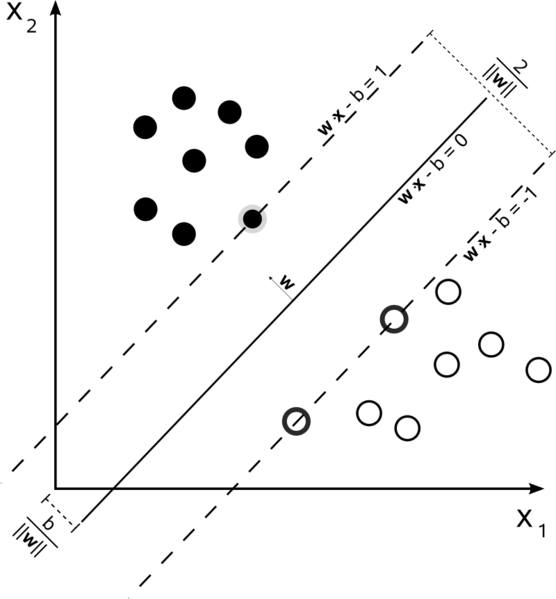
\includegraphics[width=0.5\textwidth]{Svm_max_sep_hyperplane_with_margin.png}
\caption{Margins for an SVM trained with samples from two classes}
\label{fig:svm_margin}
\end{figure}

This distance from the decision surface to the closest data point determines the margin of the classifier.

Therefore, the decision function for an \Acrshort{svm} is fully specified by a (usually small) subset of the data which defines the position of the separator, which can be seen in figure \ref{fig:svm_margin}. These points are referred to as the support vectors. They are called vectors because in a vector space, a point can be thought of as a vector between the origin and that point.

\subsection{Hybrid Systems} % (fold)
\label{sec:other_approaches}






\section{Summary} % (fold)
\label{sec:related_work_summary}


Park’s Vector Approach to detect an inter turn stator fault in a doubly fed induction machine by a neural network 

Recent Advances in Modeling and Online Detection of Stator Interturn Faults in Electrical Motors
